% Created 2014-07-28 Mon 12:55
\documentclass[11pt]{article}
\usepackage[utf8]{inputenc}
\usepackage{lmodern}
\usepackage[T1]{fontenc}
\usepackage{fixltx2e}
\usepackage{graphicx}
\usepackage{longtable}
\usepackage{float}
\usepackage{wrapfig}
\usepackage{rotating}
\usepackage[normalem]{ulem}
\usepackage{amsmath}
\usepackage{textcomp}
\usepackage{marvosym}
\usepackage{wasysym}
\usepackage{amssymb}
\usepackage{amsmath}
\usepackage[version=3]{mhchem}
\usepackage[numbers,super,sort&compress]{natbib}
\usepackage{natmove}
\usepackage{url}
\usepackage{minted}
\usepackage{underscore}
\usepackage[linktocpage,pdfstartview=FitH,colorlinks,
linkcolor=blue,anchorcolor=blue,
citecolor=blue,filecolor=blue,menucolor=blue,urlcolor=blue]{hyperref}
\usepackage{attachfile}
\author{John Kitchin}
\date{\today}
\title{Why org-mode?}
\begin{document}

\tableofcontents


\section{Title slide\hfill{}\textsc{slide}}
\label{sec-1}
\begin{minted}[frame=lines,fontsize=\scriptsize,linenos]{emacs-lisp-slide}
(org-show-animate '("Why org-mode is awesome!" "http://orgmode.org" "John Kitchin"))
\end{minted}
\section{Fabulous outline mode\hfill{}\textsc{slide}}
\label{sec-2}

org-mode is superb for outlining and structured text.

\subsection{Introduction}
\label{sec-2-1}

Org mode is for keeping notes, maintaining TODO lists, planning projects, and authoring documents with a fast and effective plain-text system.

\url{http://orgmode.org}

Use TAB, and S-TAB to collapse and expand headings.

Fast navigation
Put cursor at first character of headline. Use speed commands for easy navigation and action

n next visible headline
p previous visible headline
c cycle visibility

j jump - interesting, takes some getting used to
? see what else you can do

Or use your mouse for some of these
\subsection{Methods}
\label{sec-2-2}



\subsubsection{Change levels easily}
\label{sec-2-2-1}

Put cursor on a headline, and use M-right M-left to change the headline level

Use M-S-right and M-S-left to change all levels in subtrees

With speed commands
r demote subtree
l promote subtree
R demote subtree and all subsubtrees
L promote subtree and all subsubtrees

\subsubsection{Rearrange levels easily}
\label{sec-2-2-2}
Put cursor on a headline, and use M-up and M-down to change the order of headlines

With speed commands
U move subtree up
D move subtree down

\subsubsection{Conclusions}
\label{sec-2-2-3}
Org-mode is \textbf{very} good at outlines.

\subsubsection{Navigation is pretty sweet}
\label{sec-2-2-4}
Put cursor here: <- Press C-c \% to remember the location.

Move somewhere else to check something. Press C-c \& to get back there.

\section{Task management                                 :sli}
\label{sec-3}
org-mode is also phenomenal for task management.

How? TODO, deadlines and the agenda.

\subsection{{\bfseries\sffamily DONE} prepare this talk}
\label{sec-3-1}
\subsection{{\bfseries\sffamily DONE} give this talk}
\label{sec-3-2}
\subsection{Checkboxes [3/3]}
\label{sec-3-3}
\begin{itemize}
\item $\boxtimes$ task 1
\item $\boxtimes$ task 2
\item $\boxtimes$ task 3
\end{itemize}

\section{Task deadlines and the agenda\hfill{}\textsc{slide}}
\label{sec-4}

\subsection{{\bfseries\sffamily TODO} Finish this talk}
\label{sec-4-1}
\subsection{{\bfseries\sffamily TODO} Publish to youtube}
\label{sec-4-2}
It is easy to change the dates with shift-arrow keys. Put your cursor on a part of the data and use S-up and S-down to change the date.

\subsection{Check your agenda}
\label{sec-4-3}

Type C-c a < a to see an agenda for this file.

With cursor at beginning of headline:
< to narrow to headline
v to create agenda, then press a to get TODO items with deadlines
\section{Capture tasks as they come in\hfill{}\textsc{slide}}
\label{sec-5}
\begin{itemize}
\item You are working on something, maybe giving a talk

\item Suddenly the phone rings, it is the President of the United States

\item You want to take notes on the conversation, but you do not want to interrupt your work setup

\item Capture to the rescue. Type C-c c

\item select the template, fill it out, Type C-c C-c and back to work.
\end{itemize}

\section{Tags and Properties\hfill{}\textsc{slide}}
\label{sec-6}
org-mode allows you to tag headlines, and set properties on them.

Let us see how that might be helpful

\url{file://c:/users/jkitchin/Dropbox/org-mode/contacts.org}

You type C-c a m
and then you can filter by tags. 

Or try EMAIL=\{kitchin\} to find an entry with an EMAIL property that matches kitchin

Speed commands
Put cursor at beginning of headline
/ create a sparse tree based on search

\section{Links, links, links\hfill{}\textsc{slide}}
\label{sec-7}

places in the document: \ref{end} or sections: \texttt{some subsection}. Good for document navigation.

files: \url{blog.org} at line 415
\href{blog.org}{\url{blog.org} functions in emacs-lisp} or to a headline

urls: \url{http://kitchingroup.cheme.cmu.edu}

Info link: \url{org#Hyperlinks}

Link to an email in gnus:
\href{nntp\%2Bnews.gmane.org:gmane.emacs.orgmode#87ioo17zje.fsf@ericabrahamsen.net}{\url{nntp+news.gmane.org:gmane.emacs.orgmode#87ioo17zje.fsf@ericabrahamsen.net}}

Citations: \cite{mehta-2014-ident-poten} or \url{10.1021/am4059149}

\cite{calle-vallejo-2013-number,hallenbeck-2013-effec-o2,mao-2013-inter}
\subsection{some subsection}
\label{sec-7-1}

This is called a "radio target" \label{end}. You can make links to them to jump around quickly.

\section{Inline images\hfill{}\textsc{slide}}
\label{sec-8}

You can have images inline, and see them.

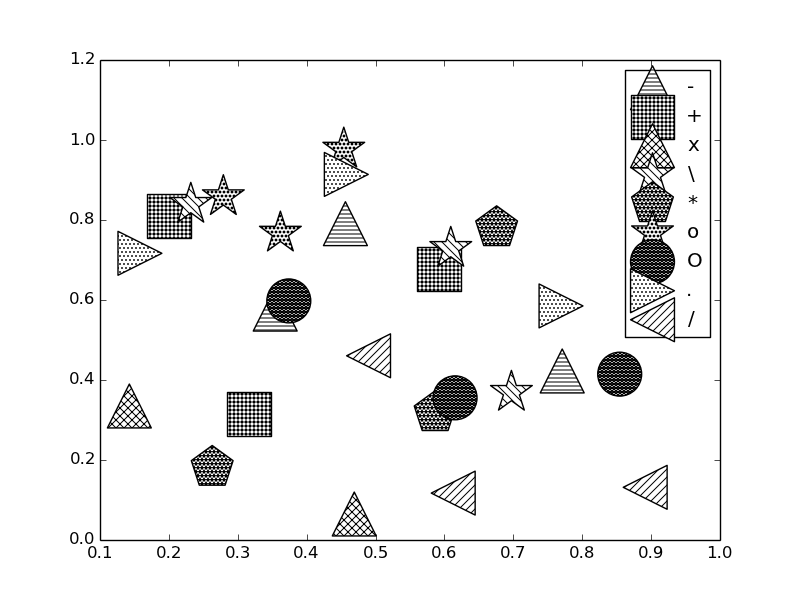
\includegraphics[width=.9\linewidth]{./images/hatched-symbols.png}

\section{Tables}
\label{sec-9}
\subsection{Creating tables\hfill{}\textsc{slide}}
\label{sec-9-1}

So easy. Start with | at the beginning of a line.

\begin{center}
\begin{tabular}{ll}
x & y\\
12 & 34\\
2 & 4\\
jfds & fjkdsla\\
3 & 8\\
a & ffjdkslafjksdlafjksdla;\\
 & \\
\end{tabular}
\end{center}
Move around and realign your table with TAB and S-TAB,

\subsection{Have a table with wide columns?\hfill{}\textsc{slide}}
\label{sec-9-2}

\begin{center}
\begin{tabular}{rl}
number & text\\
0 & A very long sentence that takes up space\\
1 & a short one\\
\end{tabular}
\end{center}

Shorten the column for readability with <n>. Want numbers left justifed? use <l>
\begin{center}
\begin{tabular}{ll}
number & text\\
0 & A very long sentence that takes up space\\
1 & a short one\\
 & \\
\end{tabular}
\end{center}

\subsection{Sorting tables\hfill{}\textsc{slide}}
\label{sec-9-3}

org-table-sort-lines, alphabetically, or numerically , in ascending or descending order.

If you do that a lot, remember C-c \^{}

\begin{center}
\begin{tabular}{rr}
x & y\\
\hline
9 & 8\\
4 & 2\\
2 & 7\\
1 & 2\\
\end{tabular}
\end{center}

Don't forget M-arrows to move rows and columns around!

\subsection{Delete and add rows and columns\hfill{}\textsc{slide}}
\label{sec-9-4}

org-table-insert-row      M-S-down
org-table-kill-row        M-S-up
org-table-insert-column   M-S-right
org-table-delete-column   M-S-left

\begin{center}
\begin{tabular}{lrl}
x & y & \\
\hline
test & 2 & \\
John & 2 & \\
Erin & 7 & \\
Andy & 2 & \\
Zoe & 1 & \\
\end{tabular}
\end{center}

\subsection{Convert a region to a table}
\label{sec-9-5}

Have a csv dataset you want to convert to a table: Select it and run M-x org-table-convert-region.

If you do this a lot, remember C-c |

And you can add a horizontal line below your cursor with C-c -

x, y
1, 3 
3, 4
5, 6
7, 8
8, 9

Need to know the sum of a column? Run C-c + on the column, and check the minibuffer. Paste it somewhere with C-y.

\subsection{Import a table from a data file\hfill{}\textsc{slide}}
\label{sec-9-6}
See this file \url{data.tab}

Run M-x org-table-import to insert it here.
\begin{center}
\begin{tabular}{rr}
x & y\\
\hline
1 & 2\\
4 & 2\\
2 & 7\\
9 & 8\\
\end{tabular}
\end{center}



C-c - to get that line.
\subsection{Convert table to \LaTeX{}\hfill{}\textsc{slide}}
\label{sec-9-7}

Need a quick way to convert a table to \LaTeX{} code?

Highlight the region and run C-c C-e C-b l L to get the \LaTeX{} code

\begin{center}
\begin{tabular}{lr}
x & y\\
\hline
John & 2\\
Erin & 7\\
Andy & 2\\
Zoe & 1\\
\end{tabular}
\end{center}

Want HTML instead?  C-c C-e C-b h H

\section{Equations\hfill{}\textsc{slide}}
\label{sec-10}

You can put equations in your documents: $\int_0^x \sin x = 0.5$. Solve for $x$. 

Show the equation code: C-c C-c

Toggle them as images: \url{org-preview-latex-fragment} or C-c C-x C-l

Use symbols like $\propto$, or $\alpha$, with superscripts like x$^{\text{2}}$ or subscripts like CH$_{\text{4}}$. Toggle symbol overlays like this:

\url{org-toggle-pretty-entities}


\(e^x\)
\section{Embedded code}
\label{sec-11}

\subsection{Use executable code in more than one language\hfill{}\textsc{slide}}
\label{sec-11-1}

describing how to add two numbers

$e^x=5$
\begin{minted}[frame=lines,fontsize=\scriptsize,linenos]{python}
print 7 + 7
\end{minted}

\begin{verbatim}
14
\end{verbatim}




\begin{minted}[frame=lines,fontsize=\scriptsize,linenos]{common-lisp}
(+ 7 7)
\end{minted}

\begin{verbatim}
14
\end{verbatim}



\begin{minted}[frame=lines,fontsize=\scriptsize,linenos]{r}
sum(c(6, 7))
\end{minted}

\begin{verbatim}
[1] 13
\end{verbatim}



\begin{minted}[frame=lines,fontsize=\scriptsize,linenos]{perl}
print 6 + 69
\end{minted}

\begin{verbatim}
75
\end{verbatim}


\begin{minted}[frame=lines,fontsize=\scriptsize,linenos]{ruby}
print 6 + 69
\end{minted}

\begin{verbatim}
75
\end{verbatim}


\begin{minted}[frame=lines,fontsize=\scriptsize,linenos]{matlab}
% Only on Mac and Linux.
\end{minted}

What, you want inline code? You mean show that 2 + 2 = \texttt{4}. Maybe you prefer inline python: \texttt{4}.

Check out how that exports.

\subsection{Use data in a table in code\hfill{}\textsc{slide}}
\label{sec-11-2}

Tables in org-mode are sources of data. Give a table a name.

\begin{center}
\begin{tabular}{lr}
x & y\\
\hline
Erin & 7\\
John & 2\\
Andy & 2\\
Zoe & 1\\
fred & 5\\
long-nmae & 7\\
\end{tabular}
\end{center}


Use it as a variable in a code block

\begin{minted}[frame=lines,fontsize=\scriptsize,linenos]{python}
print data[0]

import matplotlib.pyplot as plt
plt.plot([int(x[1]) for x in data])
plt.show()
\end{minted}

\begin{verbatim}
['Erin', 7]
\end{verbatim}


We might as well as make a link back to our table \ref{table-data}. Go ahead, click on it.

\subsection{Make your figures in your document\hfill{}\textsc{slide}}
\label{sec-11-3}

\begin{minted}[frame=lines,fontsize=\scriptsize,linenos]{python}
import matplotlib.pyplot as plt

plt.plot([1,2,3,4])
plt.savefig('images/silly-plot.png')
\end{minted}

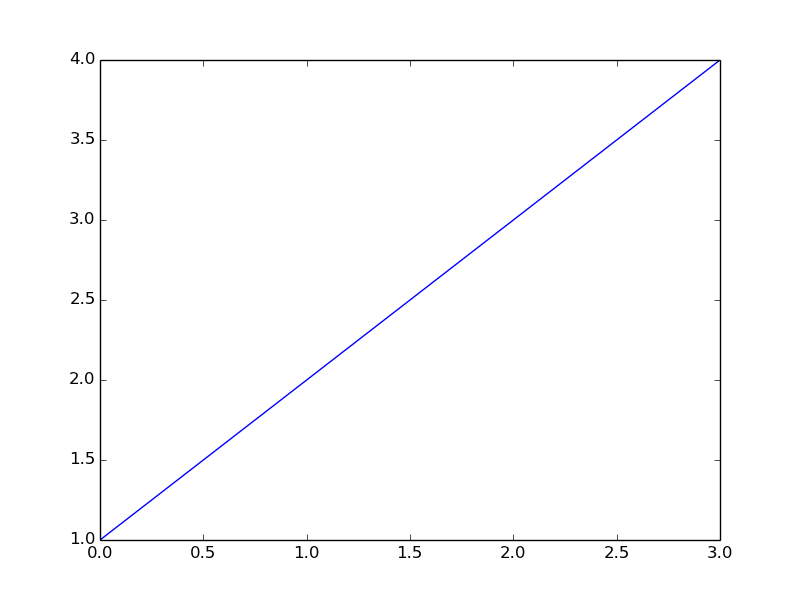
\includegraphics[width=.9\linewidth]{./images/silly-plot.png}

You can toggle inline images if you do want to see them: \url{org-toggle-inline-images}

\subsection{Write programs to your disk\hfill{}\textsc{slide}}
\label{sec-11-4}

\begin{minted}[frame=lines,fontsize=\scriptsize,linenos]{python}
print "Hello world"
\end{minted}

Tangle the file: \url{org-babel-tangle}

Now, run it:

\begin{minted}[frame=lines,fontsize=\scriptsize,linenos]{sh}
python hello_world.py
\end{minted}

\begin{verbatim}
Hello world
\end{verbatim}


check out the file: \url{hello_world.py}

\subsection{Compiled languages work too - Java\hfill{}\textsc{slide}}
\label{sec-11-5}

\begin{minted}[frame=lines,fontsize=\scriptsize,linenos]{java}
public class hello {

    public static void main(String[] args) {
        System.out.println("Hello, World from java");
    }
}
\end{minted}

Tangle the file

\begin{minted}[frame=lines,fontsize=\scriptsize,linenos]{common-lisp}
(org-babel-tangle)
\end{minted}

\begin{center}
\begin{tabular}{l}
hello.java\\
\end{tabular}
\end{center}


Compile it:
\begin{minted}[frame=lines,fontsize=\scriptsize,linenos]{sh}
javac hello.java
\end{minted}

Now, run the code.

\begin{minted}[frame=lines,fontsize=\scriptsize,linenos]{sh}
java hello
\end{minted}

\begin{verbatim}
Hello, World from java
\end{verbatim}


\subsection{C\hfill{}\textsc{slide}}
\label{sec-11-6}

\begin{minted}[frame=lines,fontsize=\scriptsize,linenos]{c}
//C hello world example
#include <stdio.h>

int main()
{
  printf("Hello world from C\n");
  return 0;
}
\end{minted}

\begin{minted}[frame=lines,fontsize=\scriptsize,linenos]{common-lisp}
(org-babel-tangle)
\end{minted}

\begin{center}
\begin{tabular}{l}
hello.c\\
\end{tabular}
\end{center}

Compile:

\begin{minted}[frame=lines,fontsize=\scriptsize,linenos]{sh}
gcc hello.c -o hello
\end{minted}

\begin{minted}[frame=lines,fontsize=\scriptsize,linenos]{sh}
./hello
\end{minted}

\begin{verbatim}
Hello world from C
\end{verbatim}





\subsection{C++\hfill{}\textsc{slide}}
\label{sec-11-7}

\begin{minted}[frame=lines,fontsize=\scriptsize,linenos]{c++}
#include <iostream>

main()
{
  std::cout << "Hello World++! ";
}
\end{minted}

You can also tangle a Makefile.

\begin{minted}[frame=lines,fontsize=\scriptsize,linenos]{makefile}
hello:	hello.c++
	g++ hello.c++ -o a.out
\end{minted}

Now, we tangle the code out to the files.
\begin{minted}[frame=lines,fontsize=\scriptsize,linenos]{common-lisp}
(org-babel-tangle)
\end{minted}



Next, we run make with the target to compile the code. You could also simply write the compiler command here.

\begin{minted}[frame=lines,fontsize=\scriptsize,linenos]{sh}
make hello
\end{minted}

\begin{verbatim}
g++ hello.c++ -o a.out
\end{verbatim}


And now get the output by running the program.

\begin{minted}[frame=lines,fontsize=\scriptsize,linenos]{sh}
./a.out
\end{minted}

\begin{verbatim}
Hello World++! 
\end{verbatim}


\subsection{Fortran\hfill{}\textsc{slide}}
\label{sec-11-8}
\begin{minted}[frame=lines,fontsize=\scriptsize,linenos]{fortran}
       program hello
          print *, "Hello World from Fortran!"
       end program hello
\end{minted}

Tangle the file

\begin{minted}[frame=lines,fontsize=\scriptsize,linenos]{common-lisp}
(org-babel-tangle)
\end{minted}

\begin{center}
\begin{tabular}{l}
hello.f90\\
\end{tabular}
\end{center}

Compile the program
\begin{minted}[frame=lines,fontsize=\scriptsize,linenos]{sh}
gfortran hello.f90 -o hello-fortran
\end{minted}

Run the program.
\begin{minted}[frame=lines,fontsize=\scriptsize,linenos]{sh}
./hello-fortran
\end{minted}

\begin{verbatim}
Hello World from Fortran!
\end{verbatim}



\subsection{There is much more language support\hfill{}\textsc{slide}}
\label{sec-11-9}

The support for editable, executable code blocks is large, and growing.

\begin{minted}[frame=lines,fontsize=\scriptsize,linenos]{common-lisp}
(directory-files "../../kitchingroup/jmax/org-mode-bleeding-edge/lisp" nil "ob-[^.]*\.el\\b")
\end{minted}

\begin{center}
\begin{tabular}{lllllllllllllllllllllllllllllllllllllllllllllllll}
ob-C.el & ob-R.el & ob-asymptote.el & ob-awk.el & ob-calc.el & ob-clojure.el & ob-comint.el & ob-core.el & ob-css.el & ob-ditaa.el & ob-dot.el & ob-emacs-lisp.el & ob-eval.el & ob-exp.el & ob-fortran.el & ob-gnuplot.el & ob-haskell.el & ob-io.el & ob-java.el & ob-js.el & ob-keys.el & ob-latex.el & ob-ledger.el & ob-lilypond.el & ob-lisp.el & ob-lob.el & ob-makefile.el & ob-matlab.el & ob-maxima.el & ob-mscgen.el & ob-ocaml.el & ob-octave.el & ob-org.el & ob-perl.el & ob-picolisp.el & ob-plantuml.el & ob-python.el & ob-ref.el & ob-ruby.el & ob-sass.el & ob-scala.el & ob-scheme.el & ob-screen.el & ob-sh.el & ob-shen.el & ob-sql.el & ob-sqlite.el & ob-table.el & ob-tangle.el\\
\end{tabular}
\end{center}

\section{Export to other formats}
\label{sec-12}
\subsection{Create \LaTeX{}/PDF from your org-file\hfill{}\textsc{slide}}
\label{sec-12-1}

see \url{file://c:/users/jkitchin/Dropbox/CMU/manuscripts/03-CuPd_paper/manuscript.org}

Gets converted to:

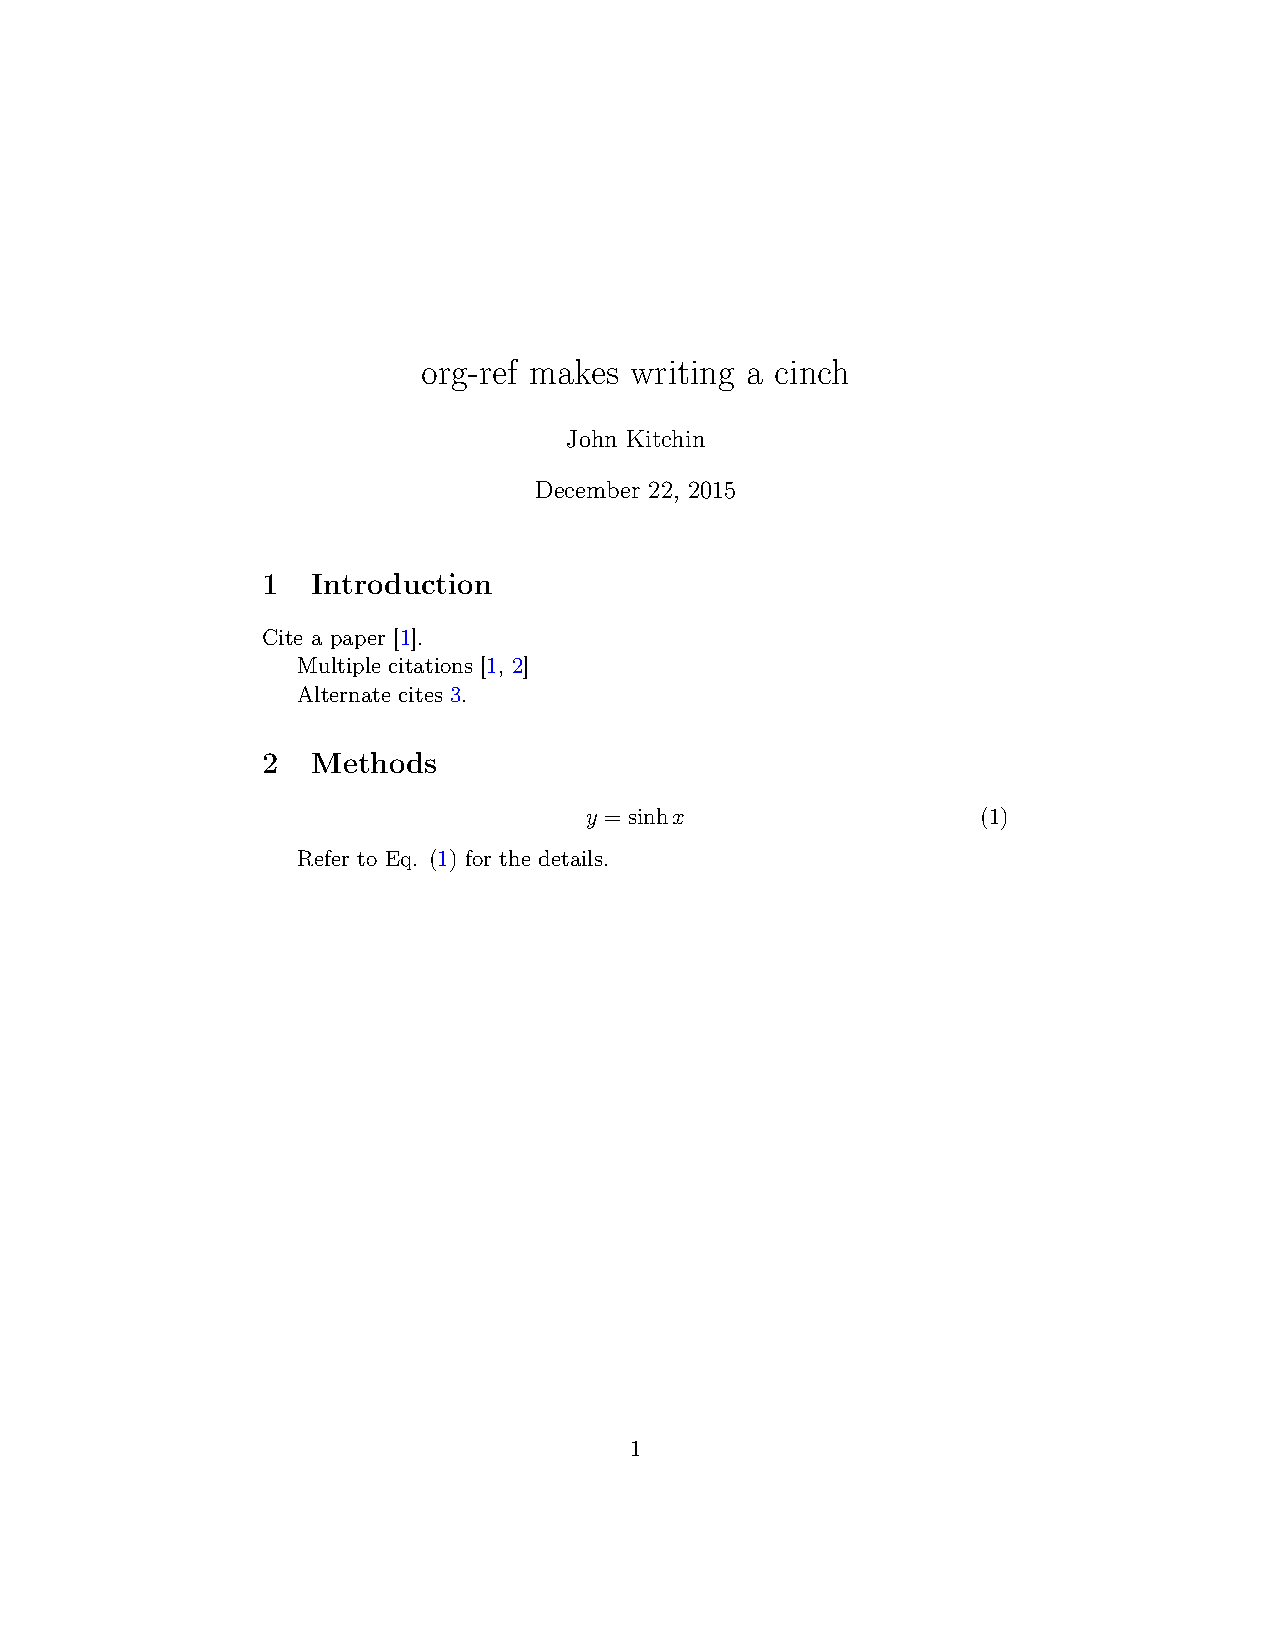
\includegraphics[width=.9\linewidth]{//c:/users/jkitchin/Dropbox/CMU/manuscripts/03-CuPd_paper/manuscript.pdf}

\subsection{Create HTML\hfill{}\textsc{slide}}
\label{sec-12-2}

We can launch this in a browser. Of course you can have \emph{italics}, \textbf{bold}, \uline{underlined}, \texttt{verbatim}, and \verb~code~.

Consider this code block:

\begin{minted}[frame=lines,fontsize=\scriptsize,linenos]{python}
a = [1, 2, 3, 4]          
b = [x**2 for x in a]     

print b
\end{minted}

That roughly is how \url{http://kitchingroup.cheme.cmu.edu} is made. We write an org-file, and export it to the blog html format.

Try it: C-c C-e h o.

\section{Extensibility\hfill{}\textsc{slide}}
\label{sec-13}
org-mode is a testament to extensibility. Checkout the \href{./../../kitchingroup/jmax/org-mode-bleeding-edge/contrib/lisp}{contrib} directory for some inspiration.

\section{Want to try it yourself?\hfill{}\textsc{slide}}
\label{sec-14}
Start out with \url{http://github.com/jkitchin/jmax}

It is pre-configured to do most of what you saw here today. For windows has a prebuilt Emacs to get started with. You have to install \LaTeX{}, python, and other languages if you are going to use them.

There are other options out there too:

I have used both of these in the past.

\begin{itemize}
\item Prelude \url{https://github.com/bbatsov/prelude}
\item Emacs-starter-kit \url{http://eschulte.github.io/emacs24-starter-kit/}
\end{itemize}

Recap: \url{(progn (widen)(require 'org-toc) (org-toc-show))}

\section{So, why aren't you using org-mode?\hfill{}\textsc{slide}}
\label{sec-15}
\begin{minted}[frame=lines,fontsize=\scriptsize,linenos]{emacs-lisp-slide}
(org-show-animate '("So" "..." "why aren't you" "using org-mode?"))
\end{minted}


\bibliography{../../bibliography/references}
% Emacs 24.3.1 (Org mode 8.2.6)
\end{document}